% Options for packages loaded elsewhere
\PassOptionsToPackage{unicode}{hyperref}
\PassOptionsToPackage{hyphens}{url}
%
\documentclass[
]{article}
\usepackage{amsmath,amssymb}
\usepackage{iftex}
\ifPDFTeX
  \usepackage[T1]{fontenc}
  \usepackage[utf8]{inputenc}
  \usepackage{textcomp} % provide euro and other symbols
\else % if luatex or xetex
  \usepackage{unicode-math} % this also loads fontspec
  \defaultfontfeatures{Scale=MatchLowercase}
  \defaultfontfeatures[\rmfamily]{Ligatures=TeX,Scale=1}
\fi
\usepackage{lmodern}
\ifPDFTeX\else
  % xetex/luatex font selection
\fi
% Use upquote if available, for straight quotes in verbatim environments
\IfFileExists{upquote.sty}{\usepackage{upquote}}{}
\IfFileExists{microtype.sty}{% use microtype if available
  \usepackage[]{microtype}
  \UseMicrotypeSet[protrusion]{basicmath} % disable protrusion for tt fonts
}{}
\makeatletter
\@ifundefined{KOMAClassName}{% if non-KOMA class
  \IfFileExists{parskip.sty}{%
    \usepackage{parskip}
  }{% else
    \setlength{\parindent}{0pt}
    \setlength{\parskip}{6pt plus 2pt minus 1pt}}
}{% if KOMA class
  \KOMAoptions{parskip=half}}
\makeatother
\usepackage{xcolor}
\usepackage[margin=1in]{geometry}
\usepackage{graphicx}
\makeatletter
\def\maxwidth{\ifdim\Gin@nat@width>\linewidth\linewidth\else\Gin@nat@width\fi}
\def\maxheight{\ifdim\Gin@nat@height>\textheight\textheight\else\Gin@nat@height\fi}
\makeatother
% Scale images if necessary, so that they will not overflow the page
% margins by default, and it is still possible to overwrite the defaults
% using explicit options in \includegraphics[width, height, ...]{}
\setkeys{Gin}{width=\maxwidth,height=\maxheight,keepaspectratio}
% Set default figure placement to htbp
\makeatletter
\def\fps@figure{htbp}
\makeatother
\setlength{\emergencystretch}{3em} % prevent overfull lines
\providecommand{\tightlist}{%
  \setlength{\itemsep}{0pt}\setlength{\parskip}{0pt}}
\setcounter{secnumdepth}{5}
\usepackage{float}
\usepackage{multirow}
\usepackage{lastpage}
\usepackage{fancyhdr}
\pagestyle{fancy}
\usepackage{booktabs}
\usepackage{longtable}
\usepackage{array}
\usepackage{multirow}
\usepackage{wrapfig}
\usepackage{float}
\usepackage{colortbl}
\usepackage{pdflscape}
\usepackage{tabu}
\usepackage{threeparttable}
\usepackage{threeparttablex}
\usepackage[normalem]{ulem}
\usepackage{makecell}
\usepackage{xcolor}
\ifLuaTeX
  \usepackage{selnolig}  % disable illegal ligatures
\fi
\IfFileExists{bookmark.sty}{\usepackage{bookmark}}{\usepackage{hyperref}}
\IfFileExists{xurl.sty}{\usepackage{xurl}}{} % add URL line breaks if available
\urlstyle{same}
\hypersetup{
  pdftitle={Exam 1},
  pdfauthor={STAT 251 Section 03},
  hidelinks,
  pdfcreator={LaTeX via pandoc}}

\title{Exam 1}
\author{STAT 251 Section 03}
\date{}

\begin{document}
\maketitle

\fancyhf{}
\thispagestyle{fancy}
\fancyfoot[L]{\textit{Instructions:} Carefully read each question. This exam is worth a total of $50$ points. For some problems, you may need to use your calculator. You should write any/all computations in the space next to the multiple choice answers for each problem. Good luck!}

\begin{table}
\centering
\begin{tabular}{cccc}

Student Name: & $\_\_\_\_\_\_\_\_\_\_\_\_\_\_$ & Last Four of Vandal Number:  & $\_\_$ $\_\_$ $\_\_$ $\_\_$ \\
&&& \\
Test Version: & \textbf{B} && \\

\end{tabular}
\end{table}

\newpage

\begin{enumerate}
\item[\bf 1.)]{ (2pts) Multiple choice: A plot which shows distinct values of a variable on the $x$-axis and the frequency or relative frequency on the $y$-axis is called a:}
\item[(a)]{Dot plot}
\item[(b)]{Pie chart}
\item[(c)]{Box and Whisker Plot}
\item[(d)]{Histogram}
\end{enumerate}

\begin{enumerate}
\item[\bf 2.)]{ (2pts) Multiple choice: A preliminary exploration and summary of the data}
\item[(a)]{descriptive statistics}
\item[(b)]{sampling design}
\item[(c)]{interquartile range}
\item[(d)]{box and whisker plot}
\end{enumerate}

\begin{enumerate}
\item[\bf 3.]{(2pts) Multiple choice: A boxplot is a visual representation of the five-number summary of a quantitative variable. Which of the following provides the correct five numbers?}
\item[(a)]{minimum, mean, range, median, maximum}
\item[(b)]{minimum, Q1, median Q3, maximum}
\item[(c)]{minimum, Q1, mean, Q3, maximum}
\item[(d)]{minimum, IQR, mean, standard deviation, maximum}
\end{enumerate}

\begin{enumerate}
\item[\bf 4.)]{(2pts) True or False: The selection of the number of bins $k$ can significantly influence the shape of a histogram}
\item[] Answer:$\_\_\_\_\_\_$
\end{enumerate}

\begin{enumerate} 
  \item[\bf 5.)]{(2pts) True or False: Inferential statistics can be applied to both samples and populations}
  \item[] Answer:$\_\_\_\_\_\_$
\end{enumerate}

\begin{enumerate} 
  \item[\bf 6.)]{(2pts) Write in the letter(s) of the words or phrases that best complete the following sentence: "The variance is a \_\_\_\_\_ of a distribution. It is \_\_\_\_\_ to outliers"}
  \item[(a)] measure of spread
  \item[(b)] susceptible
  \item[(c)] measure of location
  \item[(d)] resistant
\end{enumerate}

\newpage
\begin{enumerate} 
  \item[\bf 7.)]{(2pts) Write in the letter(s) of the words or phrases that {\underline best completes} the following sentence: "The mean is the \_\_\_\_\_ of a distribution while the median is the \_\_\_\_\_ of a distribution."}
  \item[(a)] middle value
  \item[(b)] frequency
  \item[(c)] measure of spread
  \item[(d)] center of gravity
\end{enumerate}

\begin{enumerate}
\item[\bf 8.)]{ (4pts total) consider the following sample of 3 observations of a quantitative variable $X$ 
\[ X = \{-4.4, -0.2, 1.5\}\] Answer parts (a) - (c)}
\item[(a)] (2pts) given that $\bar{x} \approx 1$, \textbf{show how to compute} the sample variance $s^2$
\item[]
\item[]
\item[]
\item[(b)] (2pts) Assuming the variance of $X$ above $s^2 \approx 9.22$, what is the standard deviation $s$? 
\item[]
\end{enumerate}

\begin{enumerate}
\item[\bf 9.)] (6pts total) The provided data originates from a survey conducted among a representative sample of 20 college students in Georgia. This comprehensive study, administered by the state, aims to explore various factors influencing academic performance concerning student behavior. As part of the survey, participants were asked to self-report the daily time they dedicate to studying in whole hours. Complete the frequency table below by providing the missing information, and address the following questions (a)-(c):
\end{enumerate}

\begin{table}[H]
\centering
\begin{tabular}{r|l|l|l}
\hline
Study Time (Hrs) & Frequency & Relative frequency & Cumulative RF\\
\hline
3 & 9 & 0.45 & 0.45\\
\hline
6 &  & 0.3 & \\
\hline
9 & 3 &  & 0.9\\
\hline
12 & 1 &  & \\
\hline
15 & 1 & 0.05 & 1\\
\hline
\end{tabular}
\end{table}

\begin{itemize}
\item[(a)]{(2pts) What kind of variable is ``Study Time (Hrs)"?}
\item[]
\item[(b)]{(2pts) Using the frequency table above, Confirm that the mean amount of time a student spends studying in this sample is $5.85$ hours}
\item[]
\item[]
\item[]
\item[(c)]{(2pts) What proportion of students study 6 hours a day or less?}
\item[]
\end{itemize}

\newpage
\begin{enumerate}
\item[\bf 10.)] (4pts total) The plot on the left shows the cumulative distribution of college grade point average from the Georgia Student Survey. Circle the letter of the boxplot that correctly depicts the cumulative distribution.
\end{enumerate}

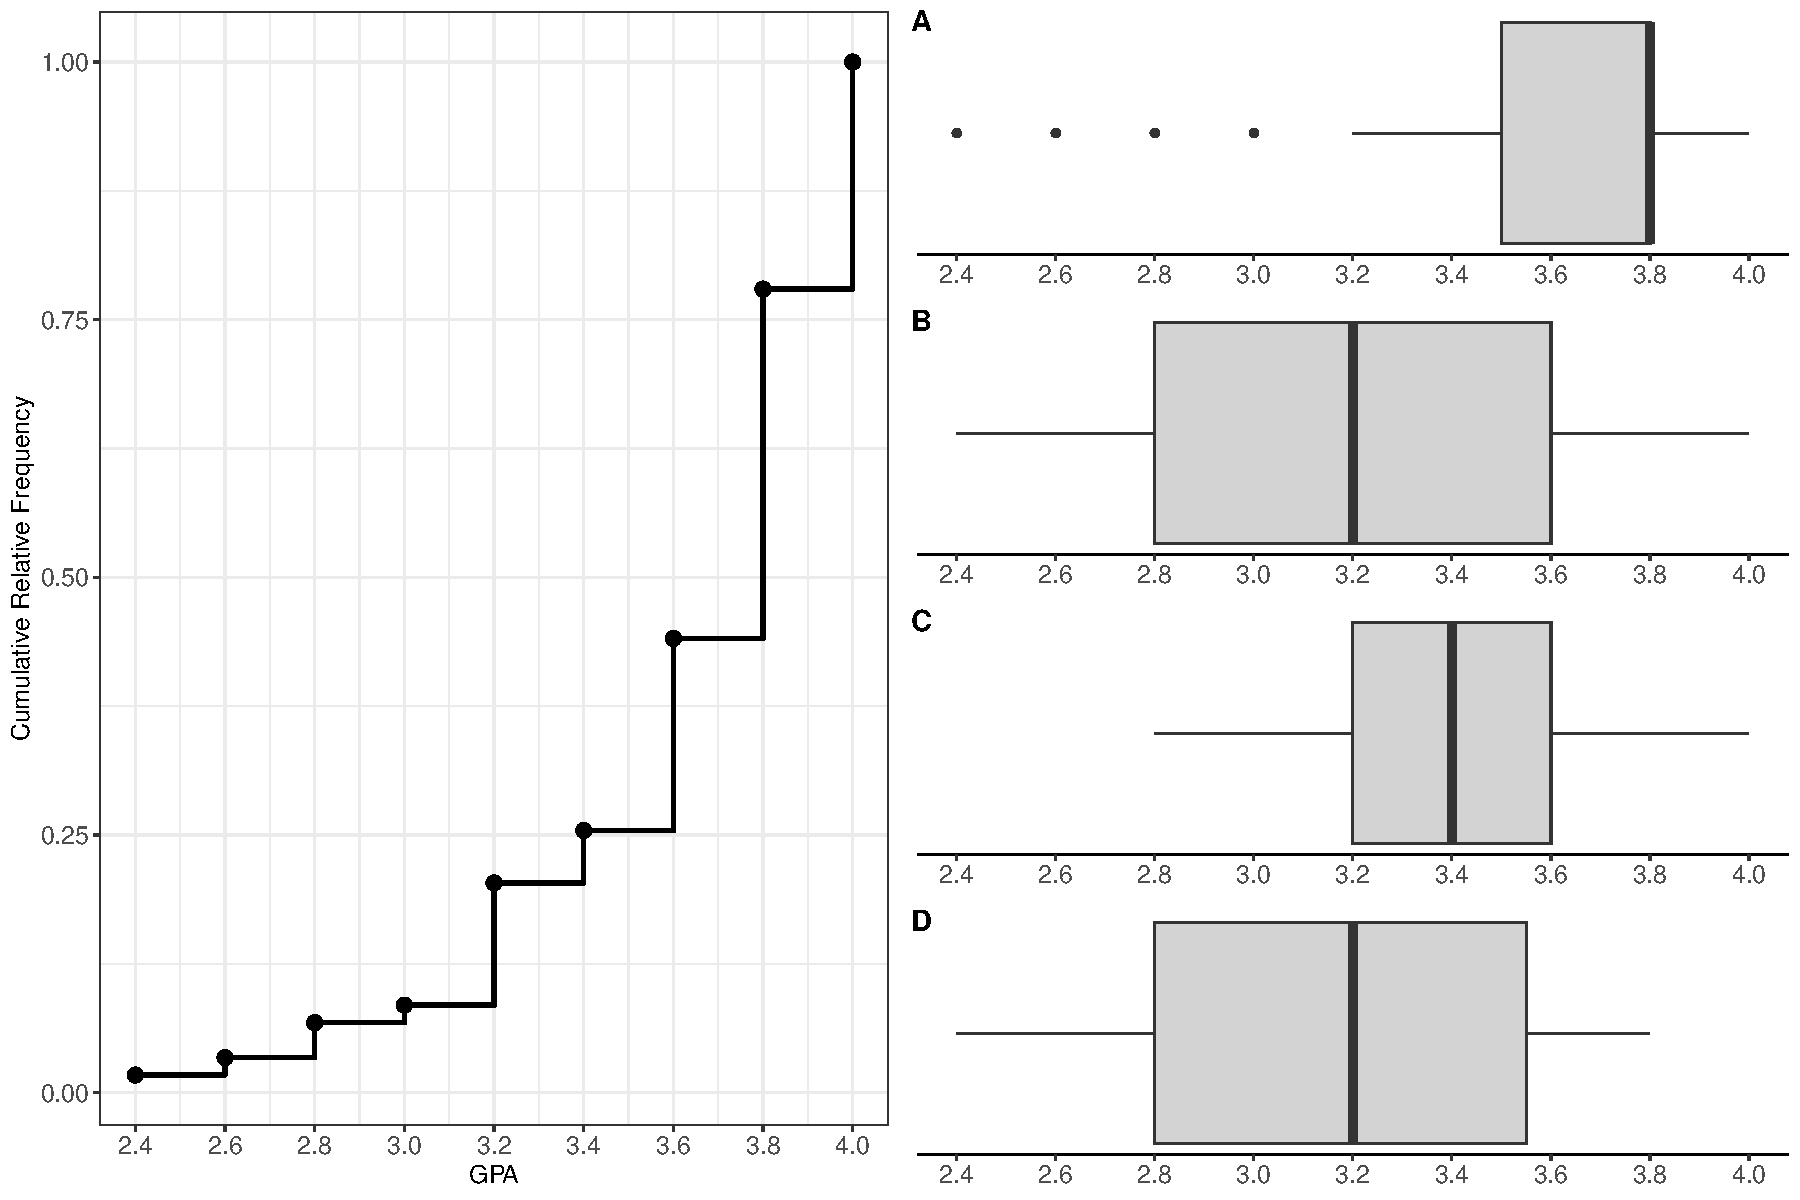
\includegraphics{Exam_1_Version_B_files/figure-latex/unnamed-chunk-2-1.pdf}

\newpage

\begin{enumerate}
\item[\bf 11.)] (6pts total) Describe the shape of the following distributions and for each distribution identify if the mean will be greater than, less than, or equal to the median (use symbols $<, \ >, \ =$).
\end{enumerate}

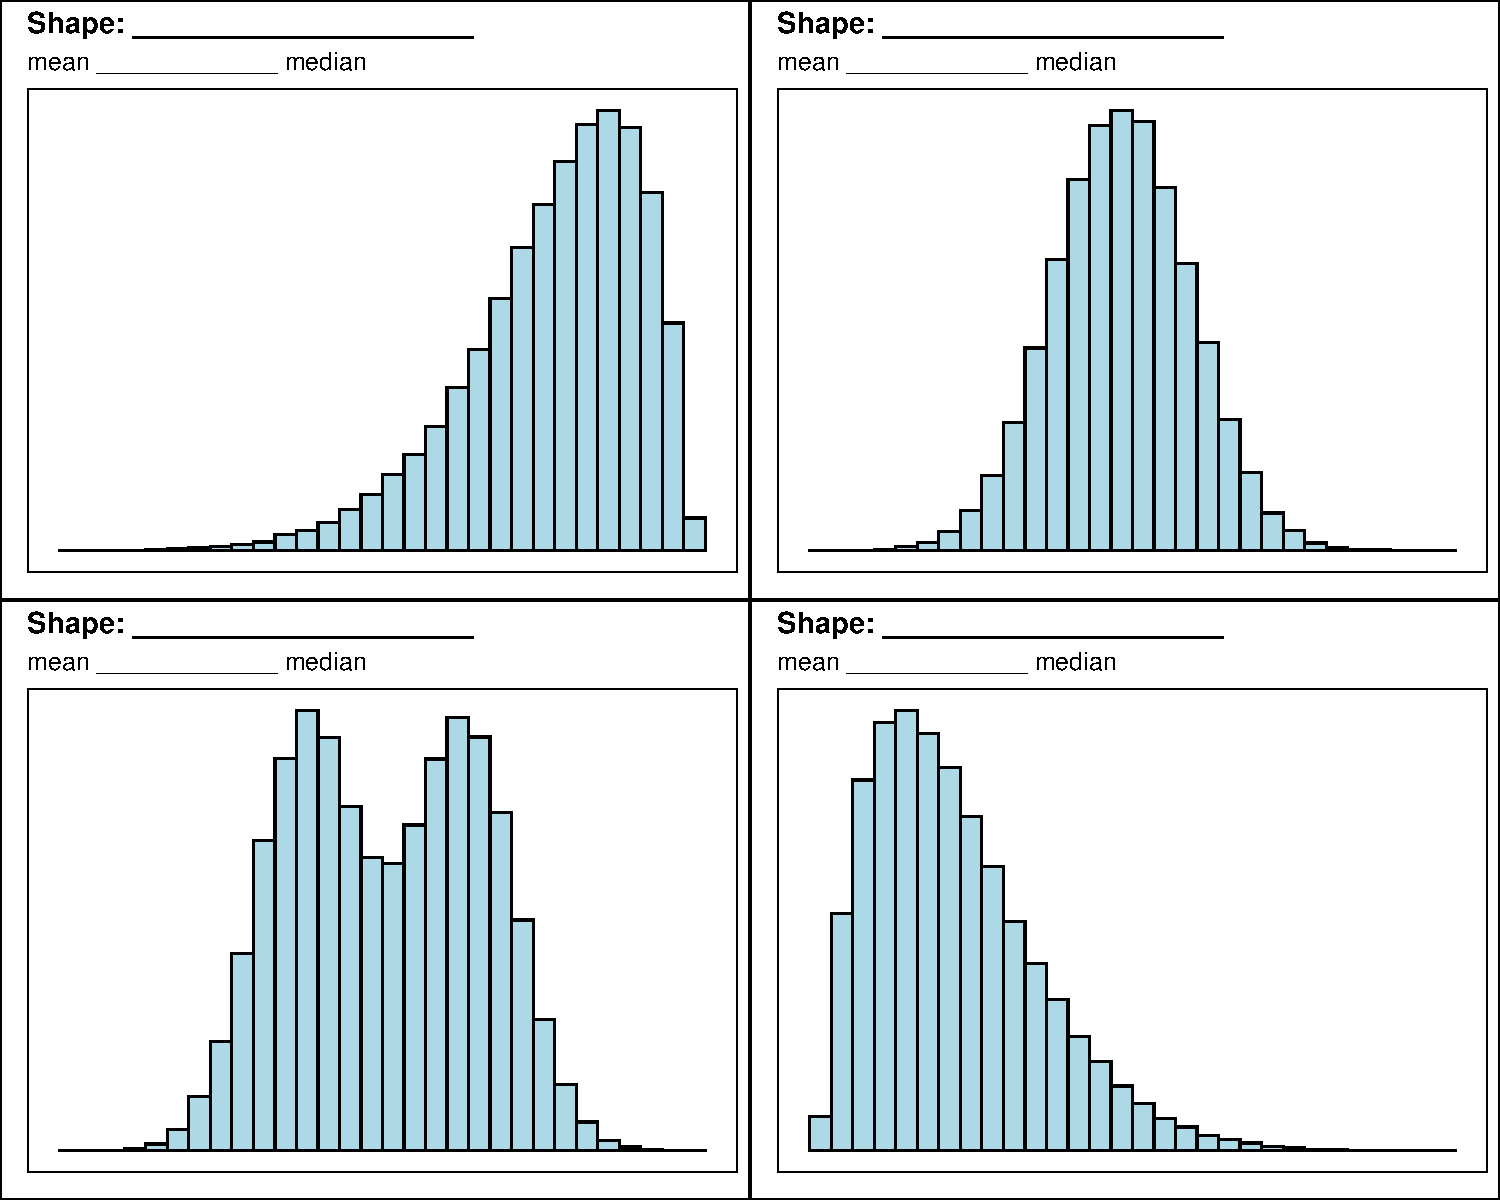
\includegraphics{Exam_1_Version_B_files/figure-latex/unnamed-chunk-3-1.pdf}

\newpage
\begin{enumerate}
\item[\bf 12.)] (4 pts total) A survey of college students in Georgia asked the following questions:
\item[A.)] Are you male or female? (recorded as male = 0, female = 1)
\item[B.)] What is you height in inches?
\item[C.)] Do you routinely smoke cigarettes? (recorded as no = 0, yes = 1)
\item[D.)] How many hours do you spend studying?
\end{enumerate}

The figure below shows histograms of the student responses to each of
these questions in scrambled order and without scale markings. Match
each variable to its corresponding histogram by indicating the
appropriate letter in the space provided on each plot.

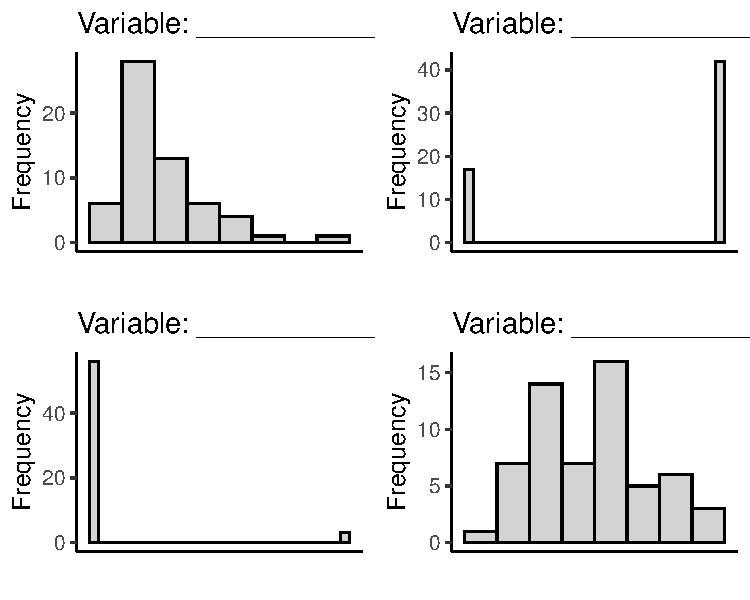
\includegraphics{Exam_1_Version_B_files/figure-latex/unnamed-chunk-4-1.pdf}

\begin{enumerate}
\item[\bf 13.)] (2 pts total) Consider the following five number summary of the sugar content in milligrams in a single serving of 20 different U.S cereal brands 
\end{enumerate}
\begin{table}[H]
\centering
\begin{tabular}{rrrrr}
\toprule
Minimum & Q1 & Median & Q3 & Maximum\\
\midrule
0 & 4 & 9.5 & 13 & 18\\
\bottomrule
\end{tabular}
\end{table}
\begin{enumerate}
\item[] Utilizing the $1.5 \times IQR$ rule and the table above, at what sugar content level does a cereal brand become classified as an outlier?
\end{enumerate}

\newpage

\({\bf (14)}\) (4pts total) Consider the following four sets of
observations of a quantitative variable \(x\). For your convenience the
observations have been sorted in increasing order. Match datasets
\(1-4\) with the correct histogram (labeled \(A - D\))
\[\text{Dataset 1} = \{0.1, 1.1, 2.6, 2.7, 3.4, 3.4, 4.1, 4.4, 8.8, 9.6\}\]
\[\text{Dataset 2} = \{1.1, 3.8, 5.3, 6.0, 6.2, 6.9, 7.9, 7.9, 8.1, 8.7\}\]
\[\text{Dataset 3}= \{0.1, 0.3, 1.2, 2.4, 4.4, 4.5, 8.0, 8.9, 9.3, 9.3\}\]
\[\text{Dataset 4} = \{3.4, 4.5, 5.4, 5.6, 7.0, 8.5, 8.9, 9.2, 9.7, 9.7\}\]
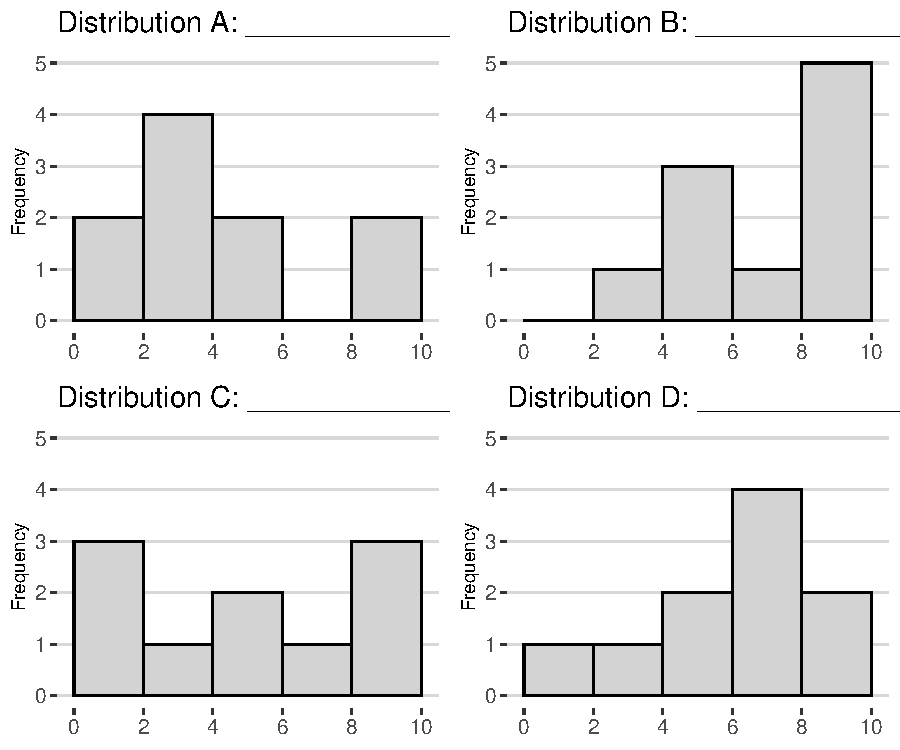
\includegraphics{Exam_1_Version_B_files/figure-latex/unnamed-chunk-6-1.pdf}

\newpage
\begin{enumerate}
\item[\bf 15.)] (6 pts total) The table below gives the distribution of a quantitative variable $X$.
\end{enumerate}

\begin{table}[H]

\caption{\label{tab:unnamed-chunk-7}}
\centering
\begin{tabular}[t]{rrrr}
\toprule
X & Frequency(X) & Relative Frequency(x) & Cumulative Relative Fequency\\
\midrule
5 & 8 & 0.40 & 0.40\\
6 & 5 & 0.25 & 0.65\\
7 & 2 & 0.10 & 0.75\\
8 & 5 & 0.25 & 1.00\\
\bottomrule
\end{tabular}
\end{table}

\begin{enumerate}
\item[]{Plot the cumulative distribution (3pts) and use this plot to find the $25th$, $50th$, and $75th$ percentiles of $X$ (1pt each)}
\end{enumerate}

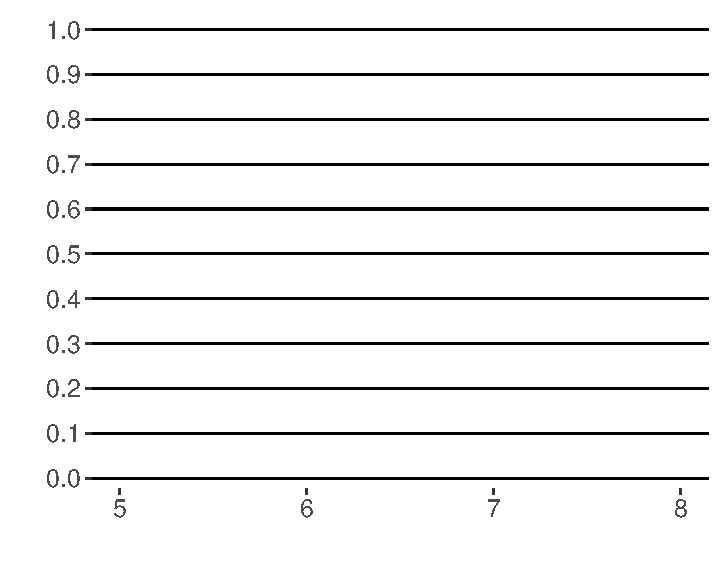
\includegraphics{Exam_1_Version_B_files/figure-latex/unnamed-chunk-8-1.pdf}

\(25th = \_\_\_\_\) \(50th = \_\_\_\_\) \(75th = \_\_\_\_\)

\textbf{Extra Credit: } Any points earned on extra credit problems will
be applied to the total score of this examination not to exceed the
total of \textbf{50} points possible.

\begin{enumerate}
\item[\bf(bonus)]{ (2pts) Why is the sample variance divided by $n-1$ instead of $n$ like the sample mean? explain you answer (a mathematical demonstration can also help)}
\item[]
\item[]
\end{enumerate}

\begin{enumerate}
\item[\bf(bonus)]{ (2pts) Why is it advisable to complement a boxplot with another type of plot, such as a dot plot or histogram, when performing a descriptive analysis of a variable? Explain the rationale behind not relying solely on a boxplot for a comprehensive understanding of the data.}
\item[]
\end{enumerate}

\newpage

END OF EXAM \newpage

\section{Formulas}

\[\bar{x} = \frac{1}{n} \sum_{i=1}^n x_i\]
\[\bar{x} = \frac{1}{n}\sum_{x} xF(x)\] \[\bar{x} = \sum_{x} xRF(X)\]
\[s^2 = \frac{1}{n-1}\sum_{i=1}^n (x_i - \bar{x})^2\]
\[s = \sqrt{\frac{1}{n-1}\sum_{i=1}^n (x_i - \bar{x})^2}\]
\[ \text{range}(x) = \text{min}(x) - \text{max}(x)\] \[IQR = Q3 - Q1 \]
\[x < Q1 - 1.5 \times (Q3 - Q1)\] \[x > Q3 - 1.5\times(Q3-Q1)\]

\end{document}
